\documentclass[a4paper, 12pt]{article}

\usepackage[portuges]{babel}
\usepackage[utf8]{inputenc}
\usepackage{amsmath}
\usepackage{indentfirst}
\usepackage{graphicx}
\usepackage{multicol,lipsum}

\begin{document}
%\maketitle

\begin{titlepage}
	\begin{center}
	
	%\begin{figure}[!ht]
	%\centering
	%\includegraphics[width=2cm]{c:/ufba.jpg}
	%\end{figure}

		\Huge{Centro Universitário Instituto de Educação Superior de Brasília}\\
		\large{Departamento de Pós graduação}\\ 
		\large{Especialização em Big Data, BI e Analytics Aplicados aos Negócios}\\ 
		\vspace{12pt}
        \vspace{70pt}
        \textbf{\LARGE{Projeto Integrador I}}\\
		%\title{{\large{Título}}}
		\vspace{3,5cm}
	\end{center}
	
	\begin{flushleft}
		\begin{tabbing}
			Aluna: Mariana Borges de Sampaio \\
			Professor: William de Almeida Silva\\
			Disciplina: Fundamentos de Big Data e Conhecimentos de Dados \\
	\end{tabbing}
 \end{flushleft}
	\vspace{1cm}
	
	\begin{center}
		\vspace{\fill}
			 Agosto\\
		 2023
			\end{center}
\end{titlepage}
%%%%%%%%%%%%%%%%%%%%%%%%%%%%%%%%%%%%%%%%%%%%%%%%%%%%%%%%%%%

% % % % % % % % %FOLHA DE ROSTO % % % % % % % % % %

\begin{titlepage}
	\begin{center}
	
	%\begin{figure}[!ht]
	%\centering
	%\includegraphics[width=2cm]{c:/ufba.jpg}
	%\end{figure}

		\Huge{Centro Universitário Instituto de Educação Superior de Brasília}\\
		\large{Departamento de Pós graduação}\\ 
		\large{Especialização em Big Data, BI e Analytics Aplicados aos Negócios}\\ 
\vspace{12pt}
        
        \vspace{70pt}
        
		\textbf{\LARGE{Projeto Integrador I}}
		\title{\large{Título}}
	%	\large{Modelo\\
     %   		Validação do modelo clássico}
			
	\end{center}
\vspace{1,5cm}
	
	\begin{flushright}

   \begin{list}{}{
      \setlength{\leftmargin}{4.5cm}
      \setlength{\rightmargin}{0cm}
      \setlength{\labelwidth}{0pt}
      \setlength{\labelsep}{\leftmargin}}

      \item Primeiro relatório do Projeto Integrador 1 da disciplina de Fundamentos de Big Data e Conhecimentos de dados.
      \begin{list}{}{
      \setlength{\leftmargin}{0cm}
      \setlength{\rightmargin}{0cm}
      \setlength{\labelwidth}{0pt}
      \setlength{\labelsep}{\leftmargin}}

			\item Aluna: Mariana Borges de Sampaio \
            \item Professor: William de Almeida Silva \

      \end{list}
   \end{list}
\end{flushright}
\vspace{1cm}
\begin{center}
		\vspace{\fill}
		 Agosto\\
		 2023
			\end{center}
\end{titlepage}
\newpage
% % % % % % % % % % % % % % % % % % % % % % % % % %
\newpage
\tableofcontents
\thispagestyle{empty}

\newpage
\pagenumbering{arabic}
% % % % % % % % % % % % % % % % % % % % % % % % % % %
\section{Introdução}

Ao longo dos anos as empresas de todos os países e de todos os continentes foram se desenvolvendo, cada um em sua área específica, sejam empresas de corretoras de seguro, empreiteiras, empresas de tecnologia, empresas de saúde, entre os mais diversos tipos e variados setores em que uma empresa pode se aplicar. Apesar dessas empresas terem conceitos e fundamentos diferentes visto que elas são pertencentes a mundos diferentes, tem-se detém um conjunto de dados, esse dado muitas vezes pode não ser estruturado, sendo ele um dado bruto, um dado que só teria sentido se fosse tratado a fim de se tornar uma informação.

Sendo assim, cada empresa existente até os dias de hoje inevitavelmente possui dado, logo possui informação. Esse dado pode ser ele armazenado em um banco de dados estruturado ou pode ser um big data, sendo este um dado não estruturado.
O big data tem por definição ser um conjunto de dados que possuem uma maior variedade, maior volume e estes dados têm uma maior velocidade. Sendo assim, o seu armazenamento é diferente do que um dado estruturado. Para isso conforme foram-se passando os anos foi sendo necessário nos meios do trabalho ter profissionais que são voltados para essa área.

\newpage
\section{Dicionário de dados e Análise de dados}
\subsection{Dicionário de dados}
A fonte de dados em questão foi extraída do Kaggle, conforme o que foi passado na dsecrição da atividade ativa.

Ao analisar o documento pode-se perceber a existência das seguintes colunas:
\begin{itemize}
    \item id;
    \item roomid/id;
    \item noteddate;
    \item temp;
    \item out/in.
\end{itemize}
A seguir, tem-se a coluna com seu respectivo significado.

\begin{itemize}
     \item id - corresponde à um valor alfanumérico que indica uma identificação única, sendo assim cada linha é um momento em que foi registrada a temperatura do edifício;
    \item roomid/id - corresponde ao nome da sala do edifício em que foi medida a temperatura. Para a identificação das medidas, tem-se o id que é um alfanumérico, visto que esses casos foram todos registrados em momentos aleatórios.
    \item noteddate - corresponde a data de anotação que foi identificada a temperatura no edifício, sendo está registrada em intervalos aleatórios;
    \item temp - corresponde a temperatura que foi atingida no edifício;
    \item out/in - indica se a classificação de cada se a temperatura medida foi no exterior ou no interior do edifício.
\end{itemize}


\subsection{Análise de dados}
Para realizar a análise de dados, foi necessário entender um pouco mais sobre o contexto do arquivo que foi extraído do kaggle. Os dados apresentados correspondem a dados oriundos de um sistema de monitoramento de temperatura da sala do edifício empresarial (admin), tanto no exterior como no interior do edifício.

Para realizar a análise dos dados foi feita a leitura do que foi apresentado a fim de entender o contexto da análise. A partir disso, foi desenvolvido um código no arquivo (ipynb) jupyter notebook que possui todo o código desenvolvido que foi criado com sessão do aplicativo juptyer notebook. Para isso, utilizei o vscode studio com a extensão referente ao juptyer notebook. Para manter o versionamento, utilizei o github, dessa forma, conforme avançava na análise e no código realizada um update no github que foi destinado a esse trabalho,https://github.com/sampaiomariana/iot-devices-data-analysis.Para o desenvolvimento do arquivo de relatório, utilizei o overleaf, que também conforme avançava foi sendo atualizado no github.

Na análise dos dados, foram seguidos cinco passos durante o desenvolvimento, sendo estes, os seguintes:
\begin{itemize}
    \item Importar os dados;
    \item Visualizar a base;
    \item Tratamento de erros;
    \item Análise inicial dos dados;
    \item Análise profunda dos dados.
\end{itemize}

Para realizar todos esses passos, foram utilizadas as bibliotecas pandas e statistics. Para realizar a primeira análise e entender o os dados, importei os dados utilizando a biblioteca pandas, dessa forma consegui ver as colunas e o conteúdo das colunas, a partir dessa primeira análise, foi possível ver que existem 97606 linhas e 5 colunas, sendo assim, tem-se 97606 registros de temperatura do edifício em momentos aleatórios.

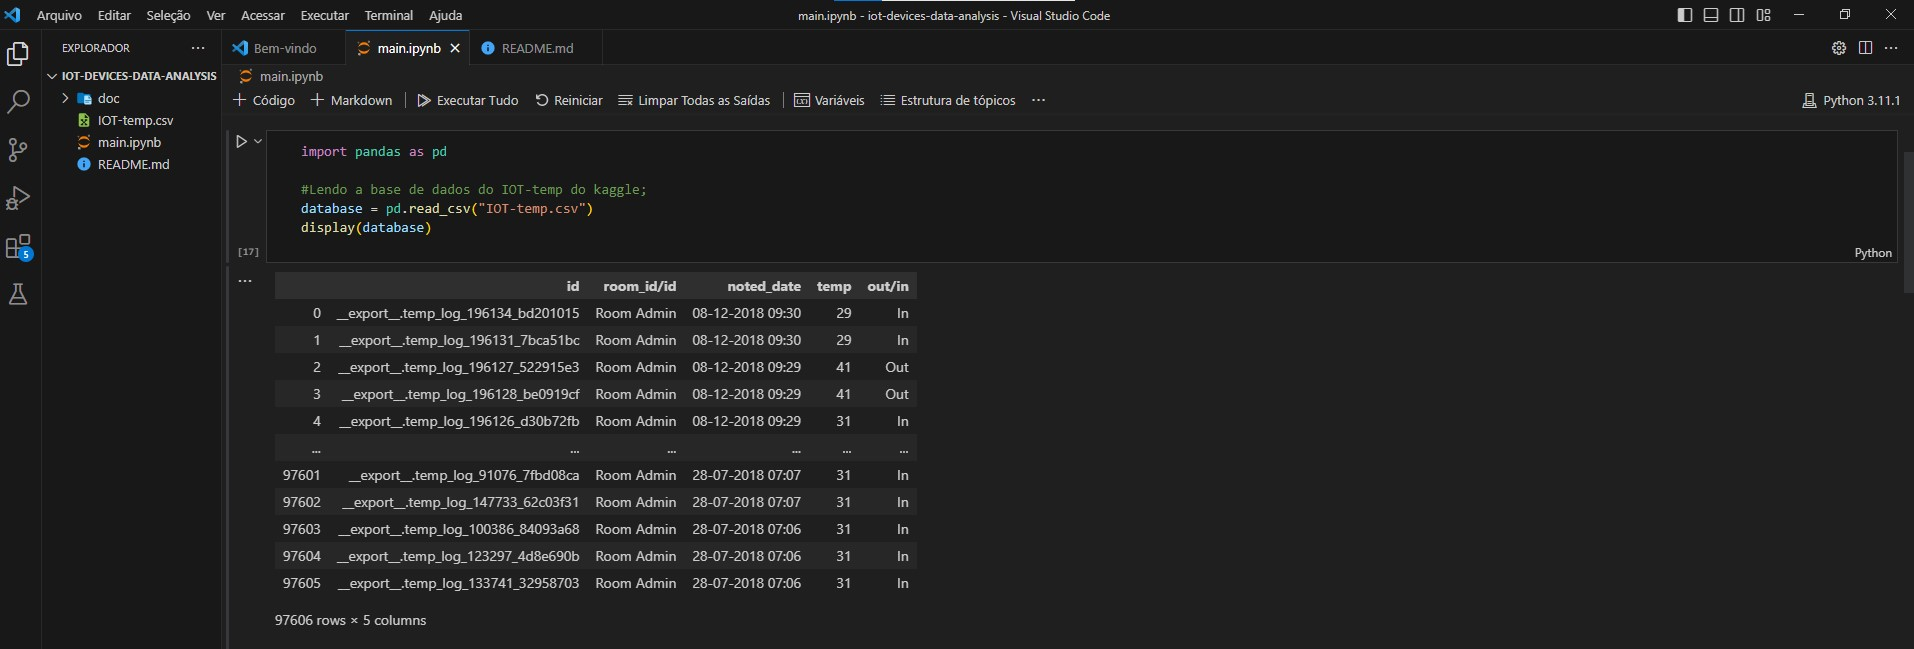
\includegraphics[scale=0.7]{img 01.jpg}

A fim de entender qual era o tipo de conteúdo em cada linha, foi feito um comando com uma descrição do conteúdo de cada linha. Essa análise é feita para ver se existem campos nulos nas colunas, caso existam eles devem ser tratados. Nesse caso, os tipos de conteúdo eram int64 e object e não existem campos nulos nas colunas. Visto que existiam duas colunas que representam a chave primária da linha, sendo ela, o id e a roomid/id, optei por retirar a coluna id.

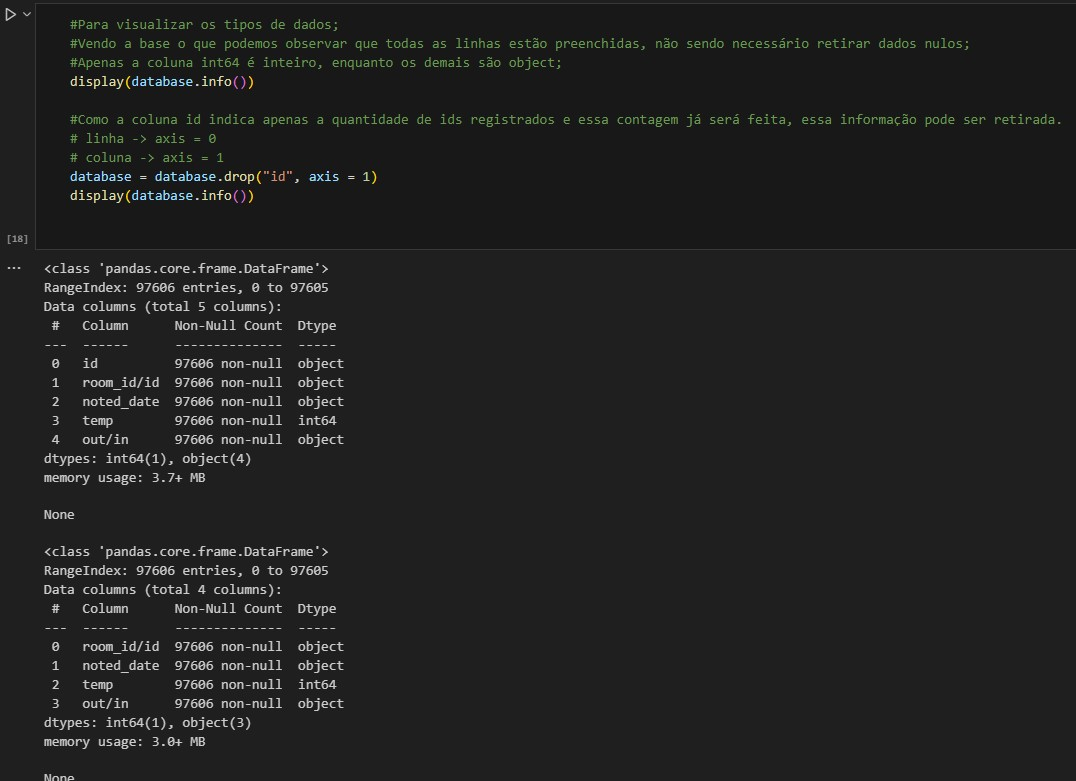
\includegraphics[scale=0.5]{img 02.jpg}
Após isso, realizei uma análise focada em cada coluna a fim de verificar na coluna do roomid/id se existia algum campo diferente de roomid, no caso da coluna de noteddate, a fim de verificar a quantidade de registros em uma data e o seu percentual. Foi possível observar que na data de 12/09/20218 tiveram mais medições de temperatura, sendo ela 65 registros, o que corresponde a 0.07 percentual do total de registros.

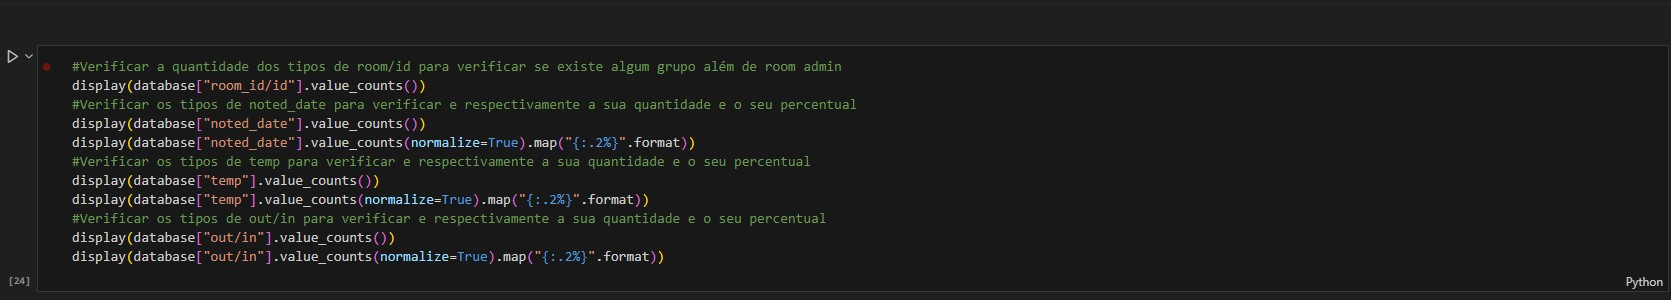
\includegraphics[scale=0.36]{img 03.jpg}

O mesmo foi feito com temp, que corresponde a temperatura, nessa análise foi possível observar que houve 10203 registros com temperatura por 39 graus, que corresponde a 10.45 percentual.

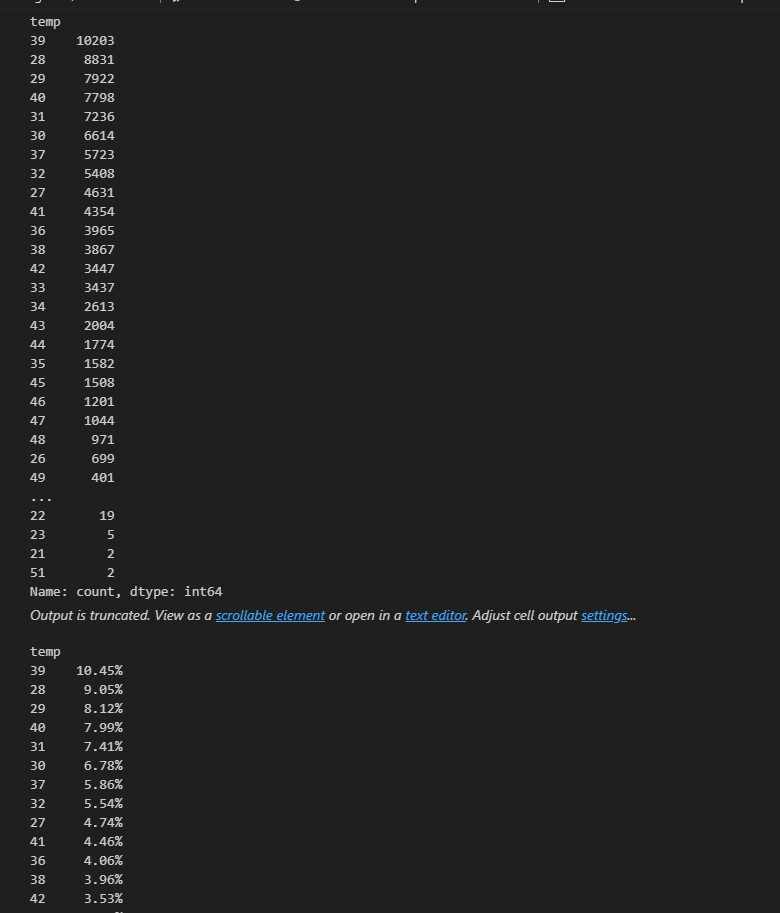
\includegraphics[scale=0.5]{img 05.jpg}

Também para a coluna de out/in foi feito, e foi possível observar que a maioria dos registros foram feitos na parte externa do edifício, pela análise, tem-se que 79.16 percentual foi medido externamente e 20.84 percentual foi medido na parte interna do edifício.

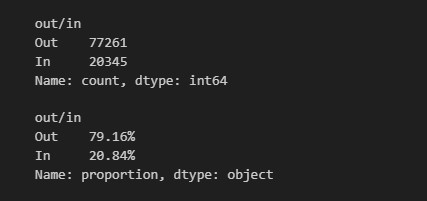
\includegraphics[scale=0.7]{img 06.jpg}

Para ter uma análise mais precisa, realizei o agrupamento dos dados, sendo baseado na coluna out/in e extrai a média da temperatura registrada, dessa forma observei que a temperatura média no lado externo do edifício foi de 36.2 graus e que no lado interno do edifício foi de 30.45 graus.

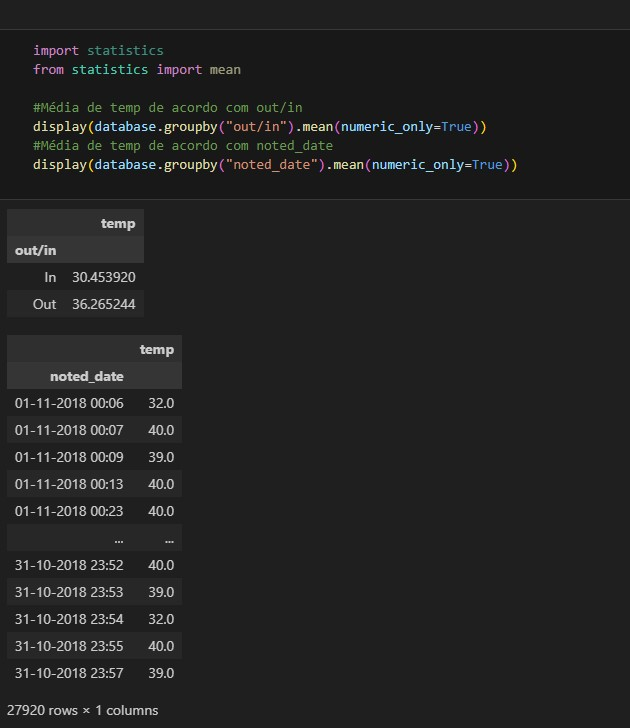
\includegraphics[scale=0.6]{img 07.jpg}

Fazendo esse mesmo agrupamento de dados, porém utilizando a coluna de noteddate como base, tem-se que a temperatura média em cada data, sendo assim, observa-se que a temperatura variou entre 32 e 40 graus durante esses dias.



\newpage
\section{Considerações finais}
Com isso, pode-se observar que ao analisar os dados, a maioria das medidas de temperatura foram feitas do lado externo do edifício, sendo possível entender que devido a exibição externa do edifício ao sol a média da sua temperatura seja maior, como indicado na análise seguinte, que apresenta a temperatura externa média de 36 graus.

Sendo assim, a análise contrária também se torna coerente, visto que apresenta dados opostos, as medidas internas apesar de serem em menor quantidade apresentam uma temperatura média menor, sendo essa de 30 graus.

Por fim, pode-se destacar a importância da análise de dados, visto que a partir dela podem ser tomadas decisões para o uso do aparelho para medição de temperatura. Nesse caso, como caso de uso, poderiam ser feitos mais registros internos também, ou até mesmo a mesma quantidade de registros poderiam ser feitas externamente a fim de obter uma média de temperatura baseado na análise das mesmas variáveis a fim de ver o comportamento da temperatura para ambos os casos.

\addcontentsline{toc}{section}{Bibliografia}
\section*{Bibliografia}
\footnotesize{

\noindent CÓRDOVA JÚNIOR, Ramiro. Introdução ao big data e internet das coisas. Disponível em: https://iesb.grupoa.education/sagah/object/default/54021327. Acesso em: 03 ago. 2023.\\

\noindent  ORACLE. O que é big data? Disponível em: https://www.oracle.com/br/big-data/what-is-big-data/. Acesso em: 02 ago. 2023.\\

\noindent MORAIS, Izabelly Soares de. Introdução ao big data e internet das coisas: introdução à ciência de dados.Disponível em: https://iesb.grupoa.education/sagah/object/default/54166276. Acesso em: 10 ago. 2023.\\
}
\end{document}



